\chapter{\textit{Archipelago}}
Creating a hybrid game using PCG represents a challenge in both design and technical areas. The hybrid game genre that has been previously defined in this paper is a recent design space to explore for designers. Even though some experiments (like \textit{False Prophets} and \textit{STARS}) or games (like \textit{XCOM: The Board Game}) already exist, exploring this concept means raising many questions about how should the digital device be integrated, and what kind of play experience is enabled by the use of PCG. The best way to answer these questions is to make a comprehensive use of prototyping.

Some results from this experiment are more related to design choices that are not depending on PCG or the hybrid nature of the game. For that reason, the creation of \textit{Archipelago} is not to be thought as a universal answer to the use of PCG in hybrid games, but more as a way to point out, illustrate and explain the challenges that appeared while creating the game. In that sense, \textit{Archipelago} only provides answers to design and technical questions in a particular framework. However, since the game has been thought from the beginning as an experimental concept, it is expected that the answers provided by the different prototypes will transcend the project presented in this paper. This means that the results that will be presented here will contribute to the exploration of making hybrid games in various ways: the successful design choices must be situated in their particular context, to recognize the patterns that support the hybrid nature of the gale; using the same approach, the experimentations that did not provide the expected results will also be analysed.

The following section will start describing the process of making \textit{Archipelago} by identifying the challenges that appeared when thinking about hybrid games using PCG. To follow, different aspects of the development process will be described in order to clearly understand the purpose of \textit{Archipelago}. Each aspect of the game is analysed in the intention to provide results both on the design and technical aspects of its creation. 
\section{Brainstorming and Game Concept Choice}
Brainstorming over the concept of hybrid game was already a challenge in itself. Because of the experimental nature of the project and the time in which the game had to be created, it was decided to focus on the key challenges that were expected, and reveal new ones all along the process.
\subsection{Prior challenges}
In order to explore the use of PCG in tabletop games, the first step was to brainstorm around what PCG could bring to the genre, and what were the pitfalls of such a combination. Based on the definition of hybrid games that was previously established and on the expectations of what PCG affords in games, the main ideas were pointed out (see appendix \ref{fig:brainstorm1}).
\begin{itemize}
\item A hybrid game is made of both digital and analogue components. The first challenge to keep in mind was that both types of components must be used for a good reason. In other words, the choice for the core mechanics must prove that the contribution of analogue components could not be simulated on a computer; the same perspective was adopted for the digital part of the game, which could not be replaced by any kind of analogue components.  
\item Another concern was to preserve the tabletop game experience, and not denature it because of hybridization. Therefore, the core concept of the game should stress out the particular element constituting such an experience. As previously stated, tabletop games cannot be reduced to the use of components, or the fact they are played on a table. The social dimension of tabletop games was the key element to stress out in order to make the analogue part of the game relevant.
\item Creating a hybrid game means comprehensively implementing a digital device to enhance the traditional game mechanics. \textit{Enhancing} does not mean creating \textit{better} mechanics. But based on the framework previously established, it was clear that the digital part of our game must "have a clear added value" (De Boer and Lamers, 2004, p.443)\cite{chap:aug}. This brings a new challenge which is tied to those above mentioned. The use of the digital component must bring something new to the tabletop game play experience.
\item The implementation of PCG must support the idea previously defined. Moreover, the concept of "replayability" (Smith et al., 2011, p.2)\cite{pdf:pcgbased} inherent to PCG-based game design must be illustrated by the game. The focus here was to make this concept visible by the players, who should understand that the game they are playing is flexible enough, so that they could replay the game without facing the same situations several times.
\item The concept of "player control" (both "direct" and "indirect") (Smith et al., 2011, p.2)\cite{pdf:pcgbased} over the procedurally generated content - linked to PCG-based game design - is also one that should be experimented thanks to hybrid games. It is one of the enhancement that was hoped to be achieved and tested throughout the project. It has been previously stated that player control is an interesting contribution of PCG-based game design, as it triggers an uncertainty related to a sufficiently varied creation of content. The players should feel that they have a certain control over the content generation, but still be surprised by unexpected outcomes.
\item This leads to "adaptability" (Smith et al., 2011, p.2). The adaptation the content to the player's actions in the game would be one of the crucial aspect of the experiment, because it shows one aspect that is hard to recreate in tabletop games without the use of computing (though certainly not impossible). However, by using a large number of parameters to feed the PCG algorithm, the content generation would provide a variety that is in this case definitely impossible to reproduce with only analogue components.
\item Finally and to stress out the core tabletop gameplay, it was necessary to be cautious about how intrusive the application would be in the game. One of the challenge while designing the game would be to provide enough information to the digital device, so that a sufficiently varied content could be generated without requesting too many inputs from the players. More generally, avoiding \textit{algorithm specific inputs} that go directly as parameters to the algorithm in order to customize it to the next state of generation was necessary. Therefore, they should be well hidden  behind the game mechanics.
\end{itemize}
Those challenges were the main ones that the project should cover. To do so first required to find a game concept based on core mechanics that would allow the exploration of those challenges.
\subsection{Concept meeting the challenges}
Based on the principles previously stated and on the related design pattern theory, a first game concept based on a core loop had to be found. The patterns had to support each other, put the players in front of dilemmas and be blended in one core loop on which the whole gameplay would be based on. 
\subsubsection{A PCG-based design pattern}
\begin{figure}[h]
    \centering
    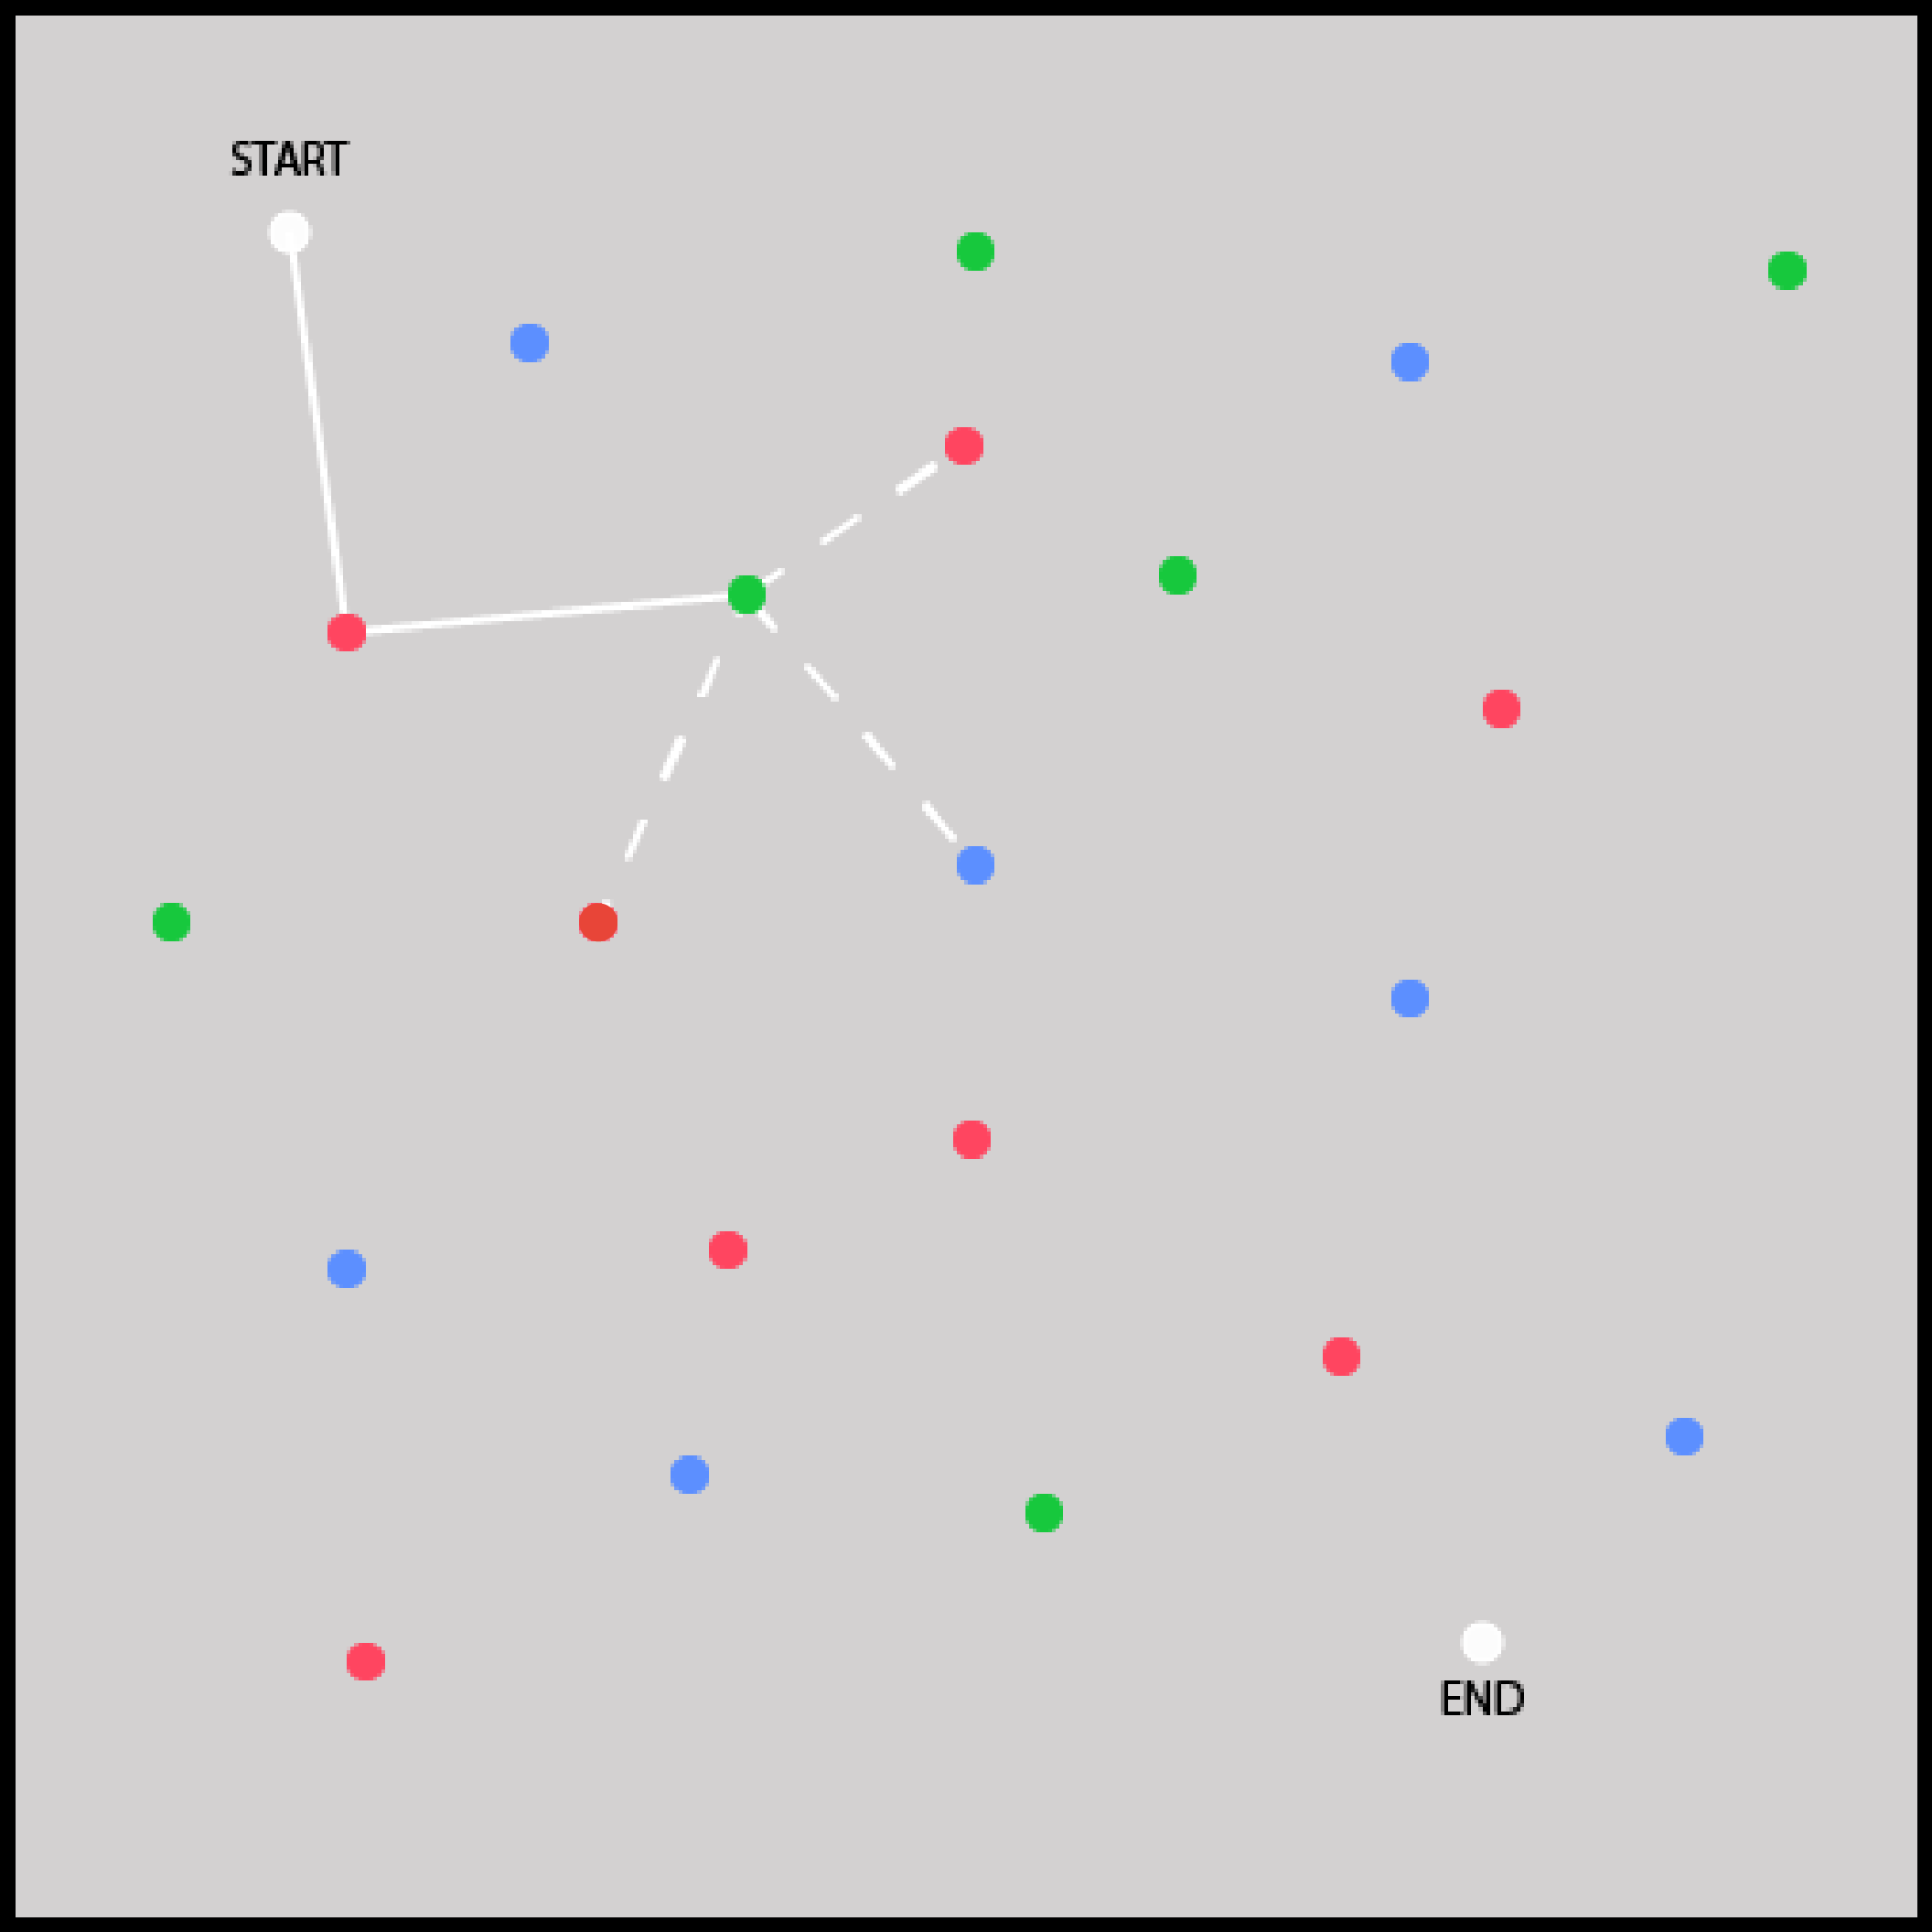
\includegraphics[scale=0.4]{Images/protomap.png}
    \caption{First map mock-up used to communicate the basic concept to the team. The nodes of different colours show the various types of locations accessible. The dotted line shows the nodes that can be reached in one move, and the full line shows the already visited nodes.}
    \label{fig:map}
\end{figure}
The first design pattern - extracted from PCG-based games - that was considered  was the \textit{Node exploration}. The player would need to explore nodes displayed on a map towards a final destination (see figure \ref{fig:map}). Examples of such mechanic can be found in \textit{FTL: Faster Than Light} \cite{game:ftl} or \textit{Out There} (Mi-Clos Studio, 2014)\cite{game:outthere} - which both inspired the creation of Archipelago. The players would have to travel or select the nodes one by one on the digital device supporting  \textit{Archipelago}'s gameplay, and progress thanks to the outcomes procedurally generated in the nodes. This pattern had several benefits, and also several implications. 

First of all, the node's content varies depending on the game, but is often based on a risk versus reward concept. The player has to foresee the potential reward that an event can provide, and balance it with the necessary risk to take in order to access it. The crucial part of this idea is to be found in the \textit{necessity} of the risk, and the \textit{possibility} of getting a reward. In \textit{FTL: Faster Than Light} \cite{game:ftl}, it is sometime a good idea to run away instead of trying to get the reward because the risk of a situation is sometimes hard to evaluate; in \textit{Out There}\cite{game:outthere} it is sometimes better to save fuel to visit more locations instead of exploiting all the planets that can be found and run out of fuel - and lose the game.

The outcomes depend on the player's choices at each node. Generally, the difficulty of the choice that the players have to make in PCG-based games enables the very specific pleasure - and sometimes frustration - of randomness. However, this kind of risk versus reward play experience is very frequently used in tabletop games (often reproduced with a dice roll). For this reason, another value should be added to this pattern, thanks to the use of PCG to create the nodes and their content. This would be included in the scope of several prototypes.

Also, this pattern naturally fits into a gameplay loop. It is a mandatory action that can overthrow a situation if the risk taken by the player is too big - in the case the player is unprepared, or if the risk was not realistically estimated. Finally mechanics based on this pattern using PCG are challenging to design because of the many possibilities that the players can be confronted to. 
\subsubsection{Board Game mechanic}
\begin{figure}[h]
    \centering
    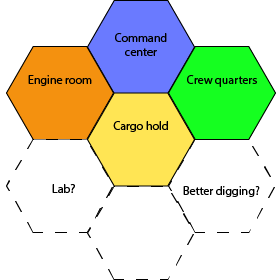
\includegraphics[scale=0.5]{Images/Base.png}
    \caption{Early mock-up describing the tiled structure of the base. Each dotted hexagon represents a possible new upgrade of the base.}
    \label{fig:base}
\end{figure}
The \textit{Base Management} pattern is the next one that was chosen to create the analogue part of \textit{Archipelago}. The term \textit{base} refers to the central part of the game, that the players would use to travel from one node to the other. This pattern is closer to tabletop game mechanics, where the players use the different resources available to progress through the game. As an example, the game \textit{Agricola} (Rosenberg, 2007) \cite{game:agri} illustrates this mechanic in various ways: the players need to improve their resources collecting capacity in order to manage their farm and their family. This create a progression based on the player's ability to manage resources correctly in order to produce more resources during the later turns in the game.

In \textit{Archipelago}, the resources would have different uses and origins. On the same principle, the various ways in which the base could be upgraded would provide a variety of gameplays and strategies, thus enforcing the "replayability" of the game.
\subsubsection{A collaborative board game}
By combining those two design patterns, \textit{Archipelago} would merge mechanics specific to PCG-based with mechanics that could well be based on a game board, although not specific to the tabletop genre. An additional element from the tabletop game definition was then required to make the physicality of the game a crucial aspect of the game, and justify its \textit{hybrid game} denomination.

Designing \textit{Archipelago} as a collaborative game was a solution to make a successful combination of board game mechanic based on tiles and exploration of locations based on PCG. One single base would be shared by all the players thus emphasizing the social dimension of tabletop games. This is one of the things that make the board irreplaceable in the case of Archipelago. The board would provide an interface around which players can gather and plan the management of the base and the allocation of the necessary resources.

The collaboration would also enhance the PCG-based mechanics of the game in an original way. Indeed, games using this mechanic leave their player alone when evaluating the risk of performing or not an action. The fact that a player is on her own when taking decision enables a very special experience - a mix of relief, frustration and regret at the same time. With \textit{Archipelago}, the players would have to take the decisions together. This different approach would also bring another kind of flavour to hybrid games, and it was hoped that the discussions that would take place before performing the events would provide an enjoyable experience, confronting the players to the failure - or success - based on a team member's decision.

The combination of those patterns was the base of the core loop (see figure \ref{fig:loop}). The players would have to collaborate managing their base using the resources found during the event exploration. The events would be procedurally generated and only occur on the digital device. Building over such an abstract game concept required another brainstorm session to explore the possibilities offered by such mechanic, and exploit the digital component using PCG (see appendix \ref{fig:brainstorm2}). The inspirations found after the brainstorm session gave directions to explore potential hybrid game specific experiences.
\begin{figure}[h]
    \centering
    \includegraphics[scale=0.5]{Images/Core_loop.png}
    \caption{The core loop and the three different steps dividing one turn.}
    \label{fig:loop}
\end{figure}
\section{Designing \textit{Archipelago}}
As mentioned earlier, the PCG integration in hybrid games on a design point of view is explored via prototypes. Based on the prototyping methods and playtest results analysis explained in section \ref{sec:proto}, the game evolved towards a final state which encompasses all the different mechanics used to prove the interest of using PCG in a hybrid game. Instead of describing the different steps of the development, the most crucial aspects of the game supporting the research purpose and the principles behind their evolution will be described in this section.
\subsection{Story}
In \textit{Archipelago}, the players have been sent by the King of their homeland to explore a newly discovered archipelago of floating islands. They are commanding a flying castle that is powered by a crystal emitting energy. The castle is composed of rooms that each have several functions in the game (both in the management phase and the exploration phase. These rooms range from \textit{Mining Guild} allowing the players to gather the required material for construction; to \textit{Mechanic's Workshop} to repair the rooms that are damaged during the exploration phase. The players have to fly from one island to the other in order to reach the final island on the map and finish the game. Islands are composed of different locations, which are generally filled with magic: magic crystals are scattered around the archipelago and with time created strange effects.

The archipelago is inhabited though, and the players will have to confront the different factions, sometimes by  allying; other times by betraying. The relation with the factions influences the outcomes in various ways, modifying the amount of resources that players gain, and affecting the game's difficulty. The events then become more and more dangerous as the players progress and acquire a reputation in the archipelago.
\subsection{Early prototyping}
In the early stages of the development, it was necessary to test the core mechanic established before moving on to the implementation of the digital device and the PCG. A first prototype was created. The purpose of this prototype was to experiment the core loop as well as the first basic mechanics around which the game would be built, and communicate this concept to the team.
\subsubsection{First iteration}
\begin{figure}[h]
    \centering
    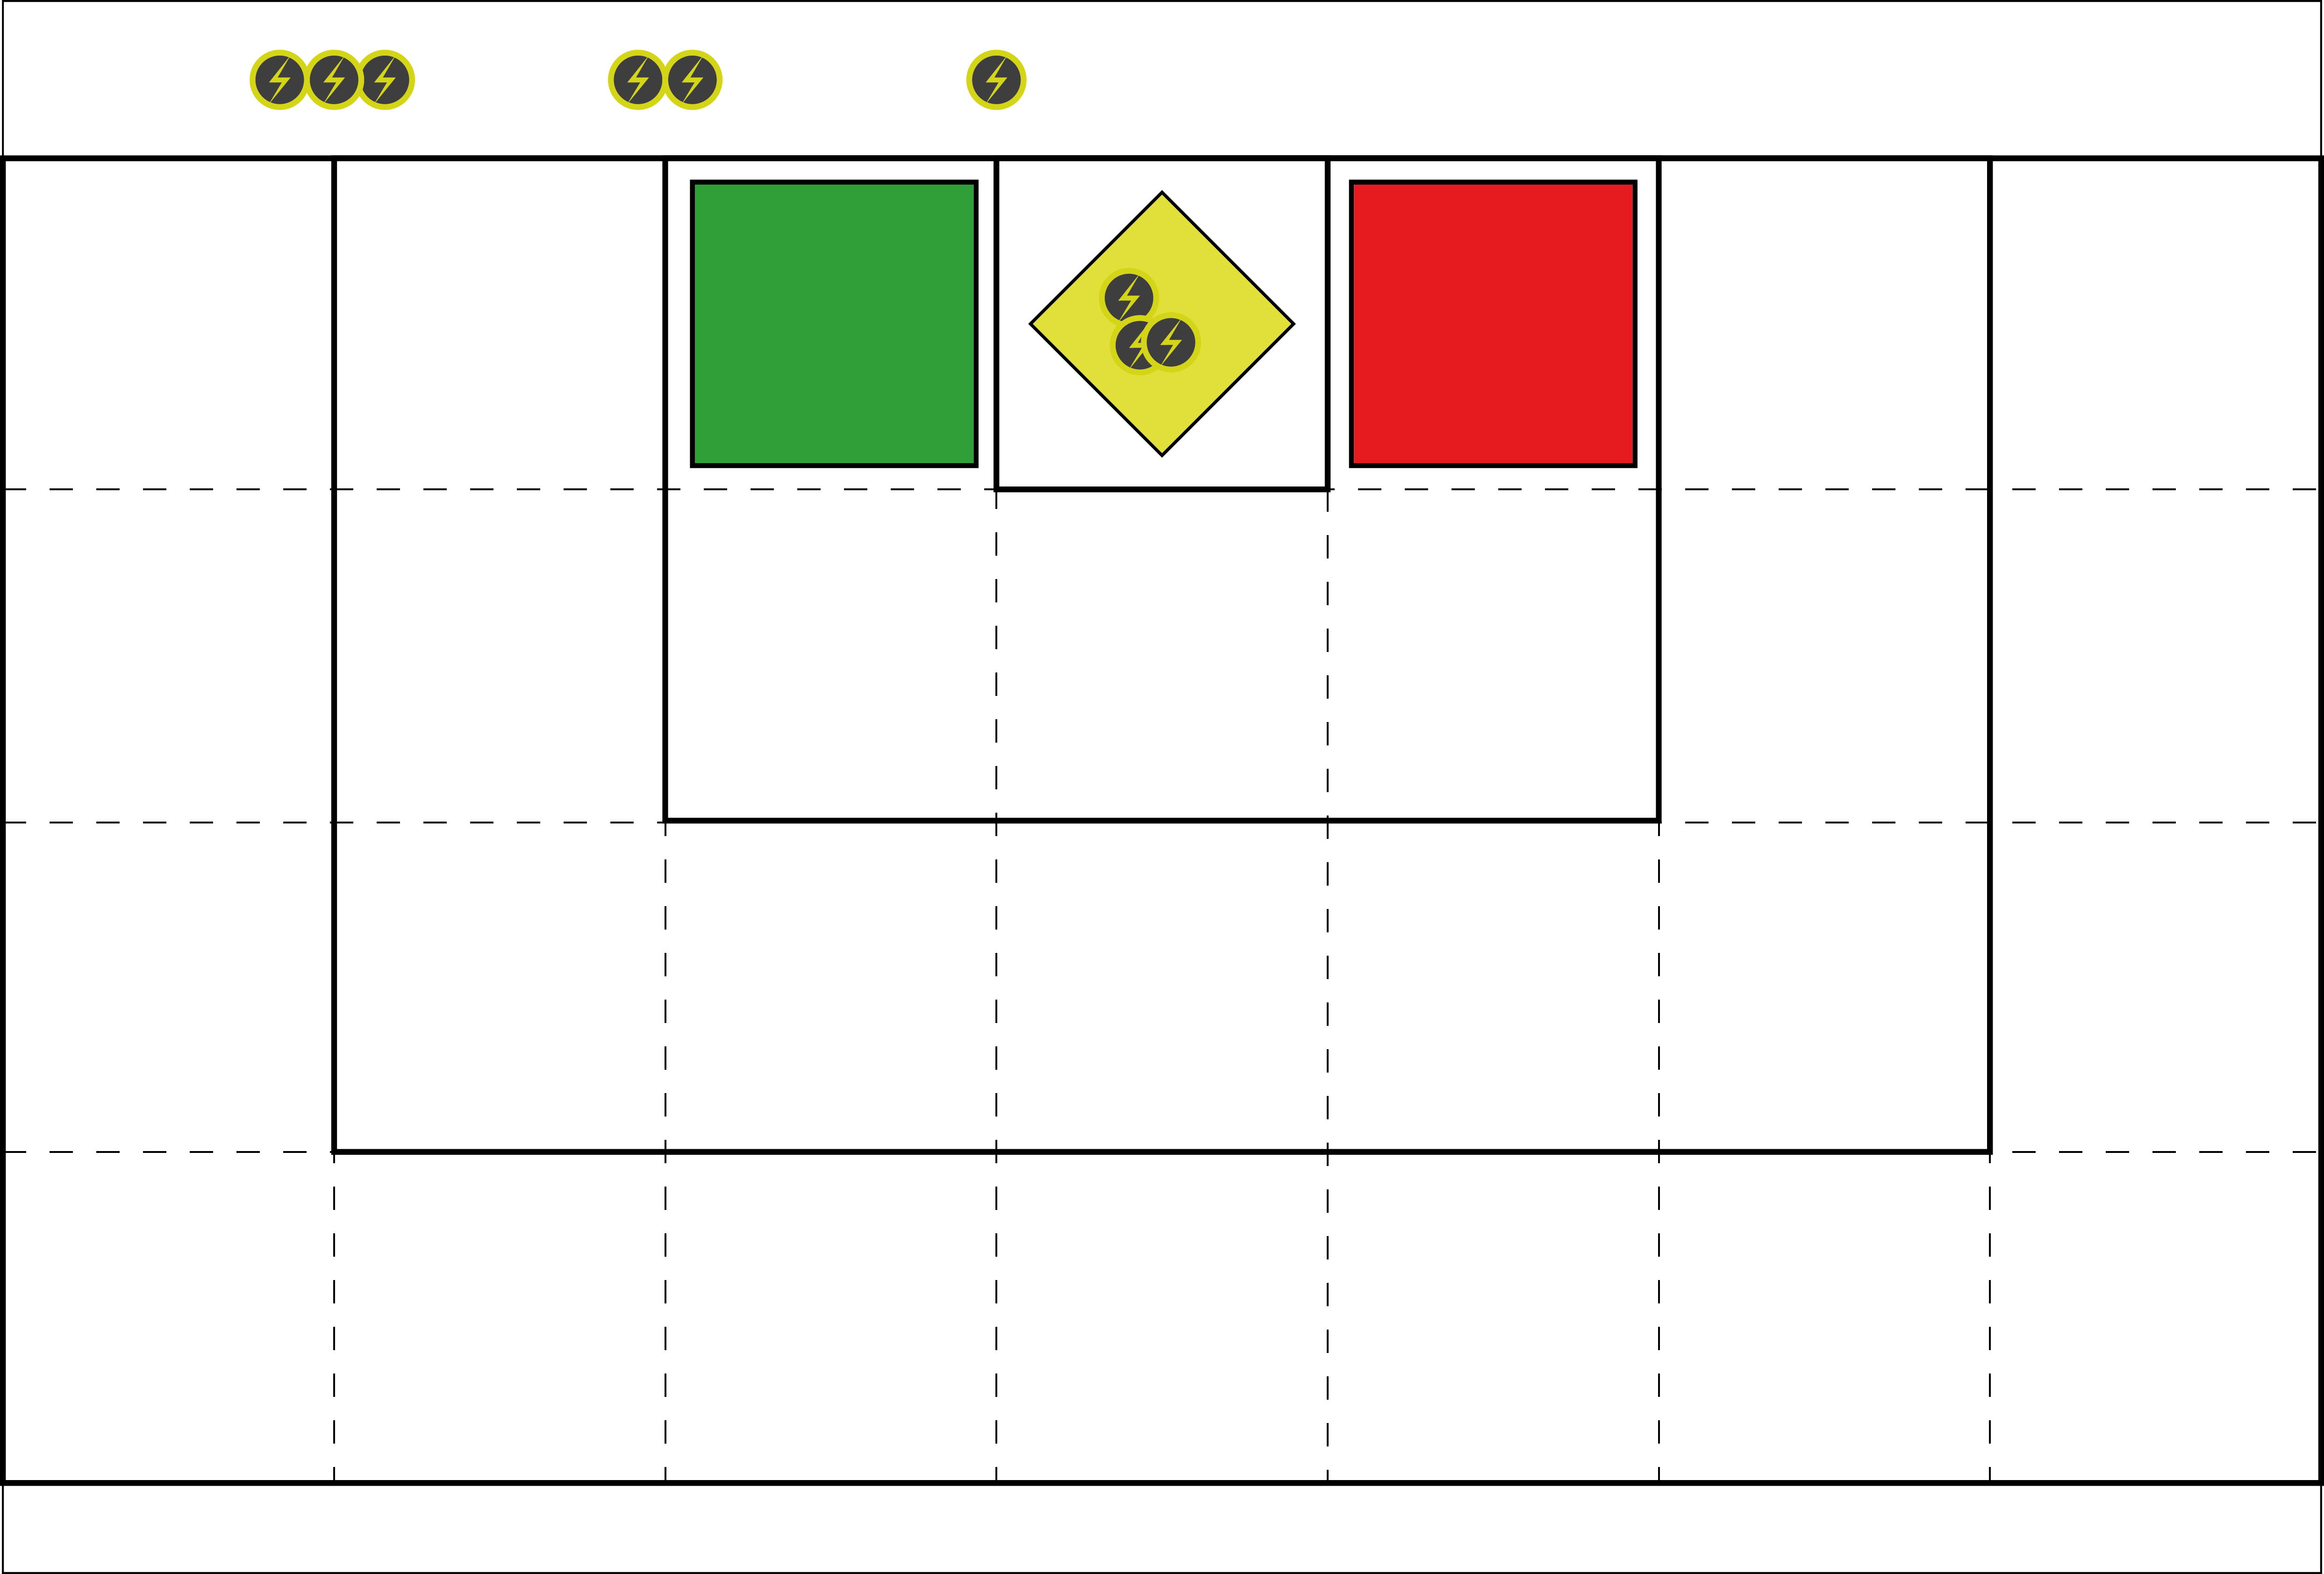
\includegraphics[scale=0.5]{Images/Board1.png}
    \caption{A representation of the base used in the first prototype.}
    \label{fig:base1}
\end{figure}
Based on Lim et al.'s framework to create relevant prototypes, the first iteration of \textit{Archipelago} is described by the \textit{main properties of prototypes}.

Since it was one of the first version to be tested by players external to the team, the application using PCG was not yet ready. Therefore paper and dice composed the \textit{Material}. The paper was used for the representation of the base on the game's board; the dice were used to simulate the PCG part. This prototype had a low-fidelity \textit{Resolution}. The representation of the base is very abstract and the digital component of the game was only simulated. The \textit{Scope} included several purposes: testing how the base should be represented on the board and how it should be managed, experimenting a basic resource system based on collaboration and providing an idea of when the digital component should be used in the game. \\\\
The mechanics of the prototype already contained several elements that still in the final game (sometimes in a different manner). Refer to figure \ref{fig:base} for each description given below:
\begin{itemize}
\item The base is divided into squares, each square being a space where building a room is possible. \textit{Construction Zones} have to be unlocked in order to extend the available construction space. To unlock a zone, the players have to power the \textit{Core} with \textit{Energy} tokens. The amount of \textit{Energy} tokens required to access a construction zone is indicated at the limit between the two zones.
\item The \textit{Cargo Hold} tile limits the \textit{Scrap} (used for construction) that players can have to 2 tokens per \textit{Cargo Hold} tile.
\item The \textit{Crew Quarters} limits the \textit{Crew members} that players can have to 2 tokens per \textit{Crew Quarters} tile.
\item \textit{Scrap} tokens, \textit{Crew member} tokens and \textit{Energy} tokens are gathered thanks to the \textit{Exploration Room}. To start gathering, the players assign a \textit{Crew member} to the \textit{Exploration Room} and roll a die. Assigning two \textit{Crew member} tokens provides a second die roll (see figure \ref{fig:Dicetable}). Gathering can only be done at the end of the turn.
\begin{figure}[h]
    \centering
    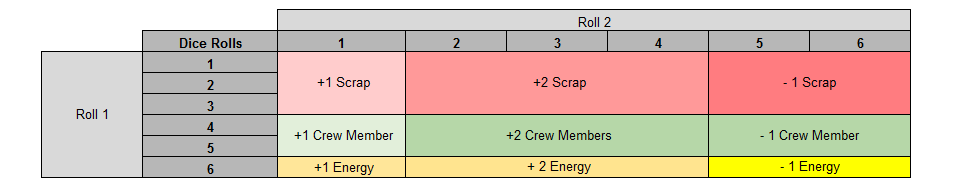
\includegraphics[scale=0.6]{Images/DiceProto1.png}
    \caption{Table representing the results of the dice rolls. One die only gives access to the leftmost column of results. A second die gives access to better rewards, but there is a risk of losing resources. There is still a chance to get a standard reward with two dice, so the risk is not necessarily worth the reward.}
    \label{fig:Dicetable}
\end{figure}
\end{itemize}
\subsubsection{Feedback}
Feedback from the first testers showed that even with abstract components, the flow of game provided a sufficiently good base for discussion. According to playtesters, dividing the board in \textit{Construction Zones} was also an interesting mechanic in itself. But it appeared several times that the players were stuck with not enough resources to play. It then needed to be refined.

The randomness of the results (due to the use of dice) also showed the problem of engagement in the game. The players were easily frustrated to lose resources because of a simple dice roll. This emphasized the notion of player control tied to PCG-based game design. Using more than one parameter proved that the players needed to feel their influence on the generation of the rewards: it happened that one player tried to convince the others that using two dice would be more efficient whereas the others thought that the risk to lose a reward was too big. Later prototypes also based on dice and paper proved that giving the possibility to influence (increasing or decreasing) the chance of getting a negative outcome could strengthen the feeling of control. This enabled more engaging discussions between the players. However, the level of abstraction showed problems of frustration.


To encourage the players to show more engagement in the game and to allow for more interesting collaboration, a specialization mechanic was built in the later prototypes. This mechanic is a crucial aspect of \textit{Archipelago} and will be described in a later section. 
 
Finally, this prototype gave a good idea of how the flow of the game would be. It was decided to build the work over this core loop to start implementing the PCG and the digital device in the game.\\\\

On the bases of the first playtest, a turn in \textit{Archipelago} would be divided in two different phases:
\begin{labeling}{Management Phase}
\item[\textbf{Management Phase}] The phase during which the players discuss and allocate the different resources in the most efficient way. This phase is based on the physical components, gathering the players around the board and using the game pieces.
\item[\textbf{Exploration Phase}] After the management phase, the players chose an island to explore on the device. This island contains locations to visit, and situations to overcome. The choices made by the players condition the amount and nature of resources they are getting. The PCG would generate the island layout, the situation that the players have to face, the options they have to face it as well as the outcome of the event.
\end{labeling}
As previously mentioned, one of the challenges of making \textit{Archipelago} was to make both digital and analogue aspects of the game support each other without interfering play as well as being essential in the game. Another important aspect justifying the purpose of this experimental game was to bring an added value thanks to the use of a digital component. PCG should bring this added value, and still be coherent with the game system. 
\subsection{Replayability}
The first aspect generally cited to enhance play with PCG-based game design is replayability, which is the idea of replaying the game without facing the same situations. The replayability of \textit{Archipelago} is supported by one of its most crucial aspect, which is to exploit PCG to generate the income of resources supporting the collaborative tabletop gameplay. The design of the event generation system was then an important part of the development and the ideas behind its evolution should be explained.
\subsubsection{An infinite number of events}
After simulating the event generation system with dice, the first iteration of the event generation system was included in the \textit{Scope} of another prototype. As observed during early prototyping, the number and quality of parameters selected to create those events and their outcomes was an important part of design. The prototype should then introduce those parameters both to the players and to the development team. Prototyping the event generation should then help manifesting two main design problems:
\begin{itemize}
\item Finding the right number of parameters to use in order to generate a content in which the patterns of the event generation system would not be recognized by the players.
\item The parameters should be intuitive for the players so that their decisions could be based on the one that they can recognize, and technically coherent so that the data could be reused for generating consistent content based on the players' actions.
\end{itemize}
It was not the first iteration implementing a digital device in the flow of the game: an iteration of the procedurally generated archipelago map layout had been tested along with the dice mechanic to further test the flow of the game (see appendix \ref{fig:gameflow}). However, it was the earliest prototype using digital components in its \textit{Material}, to generate text based events.

In \textit{Archipelago}, the events generated every time the players enter an island have several properties (see figure \ref{}). First, a text describing the situation is generated. This text depends on the \textit{location type} that the players have selected on the island. The players have several \textit{options} to face this situation. These options are only accessible to the players if they possess the required \textit{conditions} (i.e. the necessary resources or upgrades in the castle). The text describing the options is also procedurally generated. After selecting an option, a calculation is made to determine if the event was successful or not. The amount of resources collected is then determined. 
The first event generation system simply relied on a random percentage based selection of outcomes. So, the interesting part of this prototype is not to be found in its technical aspect, but in its exploration of the different parameters needed to generate coherent text based events:
\begin{labeling}{Class or Priority}
\item[\textbf{Event Type}] Three classes of event which are guidelines for their content.
\begin{itemize}
\item \textit{Gather} is related to the extraction of \textit{Scrap} (Construction Material) used to build new upgrades in the castle.
\item \textit{Research} contain events linked to resources  used to merge the different upgrades in the castle so they are more valuable.
\item \textit{Diplomacy} handles the encounters with the factions, and is a premise of what would become the later \textit{Faction System}.
\end{itemize}
\item[\textbf{Option Class}] The options available to the players to solve the events presented to him are divided into \textit{Basic}, \textit{Second} and \textit{Third}. The Events always contain options from the two first \textit{Classes}, but the \textit{Third} only has a 50\% chance of appearing. 
\item[\textbf{Risk}] The higher the class is, the better the associated maximum reward is. However, very penalizing outcomes are introduced to counter balance the rewards.
\end{labeling}
The texts of the different options and outcomes were handmade. It took a long time to reach a sufficient number of options and outcomes before testing the game. For these reasons, this method was not sufficient to prove the interest of PCG in rapidly generating content to reduce the workload of creators. Also, playtests have shown that the players could recognize the different patterns in the event generation (i.e. options showing several times in a row), thus ruining the replayable aspect of the game. However, this provided a base to work on a more complex event system:
\subsubsection{Technical flexibility and narrative coherence}
As observed during playtests of prototypes using the event generation system previously described, the generation of content was not providing enough variety to generate a potentially infinite number of events; also the workload was too high in the prospect of experimenting a sufficient amount possibilities of PCG-based game design. Solving these problems required drastic changes to attain a satisfying amount of coherent results.\\\\
A new design method for generating the events was then imagined (see section \ref{sec:eventGeneration} for the technical details).\\\\
The \textit{Outcome} is defined when performing the event. This outcome is calculated thanks to the following parameters:
\begin{enumerate}
\item The \textit{Event Type} to select the most likely resource to be collected.
\item The \textit{Condition(s)}, which is the resource(s) that the players use to access the different options available to perform the event.
\item The \textit{Class} of the option selected by the players.
\end{enumerate}
There are three types of outcomes: success, neutral or failure. The type is defined by the standard risk associated to the \textit{condition}, and the faction controlling the island. 

After an internal test, this method was selected to show the potential of PCG to create a very large number of situations and options for the players during the events. Feedback from playtesters showed that the text also needed to be carefully designed. The text needed to be coherent with the proposed options, and adaptable to a variety of situations. Therefore, the text was composed of different blocks that the digital device organizes in order to create a coherent option, understandable by the players and providing enough information regarding the risk and the potential reward. The system was also flexible enough so it was possible to experiment various rules to create the events, and increase the quantity of possible combinations. The first new implementation to try was to save data during the events in order to reuse it when the players reach another island later in the game.
\subsection{Player control and Adaptability}
In PCG-based game design, adaptibility refers to the influence of the players' actions over the generation of content. Although already covered by the event generation system, where the various options that are available to the player determine the outcomes in terms of resources gained or lost, this quality of PCG-based games needed to be emphasized in \textit{Archipelago}. 
\subsubsection{Diplomacy system}
It has already been mentioned tat early prototypes included a \textit{Diplomacy} type of events. After several prototypes using this parameter to create events, it was decided that diplomacy would be a whole system of mechanics influencing the generation of the events and the gameplay of the whole game.

The different islands of the Archipelago are inhabited by three different \textit{Factions}:
\begin{itemize}
\item The \textit{Highbournes} are described as humans native of the archipelago. They are a proud people very close to their traditions. They are the first inhabitants of the islands, and therefore have been under the magic influence of the crystals for a long time now.
\item The Nomads arrived on the Archipelago for various regions of the world. By exchanging with the Highbournes, they have acquired the rudimentary magic skills necessary to create their own transportation means and scavenge the islands for resources. They live in small villages and often confront the Humans that recently populated the archipelago.
\item The Humans are the last people who populated the Archipelago. They also arrived from various places of the world, but contrary to the Nomads, they live in large communities based on trade. Their rapid development is the primary cause of tensions between the factions of the archipelago.
\end{itemize}

The different people react differently to the players' actions. This influence is represented in the game in various ways.

First, every island is controlled by the faction. When players enter an event, they see which faction control the islands by looking at the symbol in the top left corner of the screen on the digital device. As previously explained, the faction controlling the island influences the text generated in the events (both in the options or in the text describing the situation). Until, a certain point in the development, this  

\subsubsection{Influence on the overall experience}
This system has been proposed to use the data that is saved when the players perform events
\subsection{Specialization and collaboration}
\subsubsection{Constructed Specialization}
\subsubsection{Encouraging Collaboration}
\subsection{A hybrid game}
\subsubsection{Merging Analogue and Digital}
Mainly, the function of the application is to contain all the information regarding events, movement, factions and the overall data available within the game. The application is the only connection the players will have to what is happening in the game, as without it, the game would just be an empty board with pieces that would have no purpose. 
When playing the Archipelago, the digital part of the game, the app, will provide the players with a layout of the world, i.e. the map with all its islands, and it will contain all methods of receiving rewards as well as receiving penalties for executed events. It determines which resource the players will receive, what the "story" is, in terms of flavour presented, and it contains the factions and the players standing with each of them.
The events in the app, are made to be like cards that the board game would have, if there was no app. But by having the digital computing and memory, the diversity of these events are much greater and there is no need for a huge pile of cards and expansion packs to generate different and diverse events. The app is in full control over what the players get and what is taken away from them, and given that there is now memory in place, the possibility to create new content based on previous events is there. Another part that the application plays in the entirety of the game, is that it controls when effects take place. If there has been an event with a specific outcome, it is then the system that controls if there should be consequences based on those outcomes. If there was no digital application in place, there would have to be a large amount of cards and pieces in the board game, along with very specific rules and combination guides, for the players to sufficiently be able to piece together new events and outcomes. So the biggest purpose of the app, as implemented in this solution, is to have complete control over all actions, story, events and outcomes and be able to present them to the players without using much time, which the players would do if they had to combine their own "gameplay".
\subsubsection{User Experience and Interaction Design}


\section{Development Structure (Technical)}
This part of the paper will go into more detail on how the development of the project went as seen from a more technical aspect. This includes the making of prototypes, the way to go from communicating with a designer to implementing a solution, and lastly problem solving along the way.

\subsection{From design to implementation}
When working as a developer, you also work closely with the designer. What we did during our development period, was to get the wants and needs from the designer, and try to implement it into prototypes for overlook and feedback. 
If things needed to be changed, added or removed, the team would go through in general terms what needed to be done, and then the requested adjustments would be made to the prototypes.

In the next part of this section, we will go into more detail on how the prototyping would take place, how the communication between programmers and developer happened, and what changes were made over time during the period of development.

\subsection{Prototyping (Application)}
Right from the start, it was important to quickly produce smaller prototypes so that we could get an idea of how to continue, and to test the implementations that were made. The first part of the project is to set up the app and have a starting point that you can build on. In our case, this meant an initial screen with a simple UI that could be added to, moved around and overall that could display text and data. On top of that, the backbone of the system would be to have different data classes that could contain the various sorts of information that would be needed.

\begin{description}
\item[Prototype 1:] A simple UI with text boxes, buttons and a simple data manager that contains the initial values.
\end{description}

Going onwards, designer and programmers alike, would come with inputs to set the foundation for which data types would be needed in order to produce the desired results.
It was decided early on that there would be events that the players could interact with, and that these events would have board pieces and flavour text associated with them. The basic layout for the \textit{flow} of the game is then set, with the idea that there would be a main world scene where all the destinations would be displayed, and each of these destinations would have their own scene where the locations possible would be shown.

\begin{description}
\item[Prototype 2:] Now the application has a main world screen with a multitude of destinations would be displayed in the form of simple spheres that can be clicked. When clicked, the destination scene would be shown, which contains the simple representation of locations, also in the form of spheres.
The map layout is generated by using an L-system algorithm\ref{sec:lsys}.
\end{description}

At this point, the need to link the application with the board game occurs. A player object is needed within the application, and it needs to be able to move around the world space. Also the initial event structure is taking form, which means there is a need for the data to be constructed along with some dummy flavour to be shown on the screen.

\begin{description}
\item[Prototype 3:] Introducing the player object, the event class and XML files with the initial flavour texts.
\end{description}

The events and the data contained is rather simple at this point. An event is mostly consisting of a simple description, a set of premade options, and one or two outcomes that are also premade. So a few events were made by selecting different descriptions, along with randomly selected options and an outcome for each option.

With the backbone in place for creating \textit{varying} events, the next logical step, is to start coming up with the algorithm for how the events should be constructed and generated (the actual algorithm for how it works can be seen in section \ref{sec:eve}, \textit{Events}, later in this document).

\begin{description}
\item[Prototype 4:] With a better working event generation system, the next prototype is made with a wider array of option possibilities, along with more outcomes.
\end{description}

So now the basis for the events are in place. The next part of the application, will be to have a more diverse collection of flavour texts.
This meant that we would have to come up with how the flavour text should be combined (see how in section \ref{sec:flav}, \textit{Flavour of the Events}, and in section \ref{sec:disc}, \textit{Discussion}, later in this document) and create an algorithm for doing so. 

\begin{description}
\item[Prototype 5:] Event generation is in place along with flavour-combining algorithm. Everything seems to be working as intended, with the exception of some bugs here and there. But the overall main event system that allows the first play through of the game, is now in place.
\end{description}

After going through some plays of the game, and as more design decisions are made, more functionalities have to be implemented. The next step in the prototyping cycle would be to get a faction system going. What this would mean on top of the actual faction system itself, is that there would have to be changes made to the flavour combinations, as the resulting texts would now have to include the factions. Furthermore, there would have to be special events and rewards/results from events, that would affect the reputation the players would get with the respective factions.

\begin{description}
\item[Prototype 6:]
The faction system is implemented, along with a set of special events and outcomes that can be triggered via the regular event system. Now an event can have a 3rd option, which will have the chance to trigger the special events. There are 2 types of special events implemented, the first is a faction-war event, which would let the players choose sides between factions, the second type is the big ones that are based on previous experiences and encounters that the players have had within the game. When the 2nd type of special events are selected, it will take various data from the event that triggered it and use those in special combinations to give the players the experience of \textit{history} and \textit{consequence}.
\end{description}

By now, the application has most all of the structure and algorithmic computation and generation needed to make the game a complete experience.
The remaining tasks to be solved, is implementing better visuals, icons and signifiers. Scaling the elements to fit the tablet on which it will be played, and making sure there are as little bugs as possible.

\begin{description}
\item[Prototype 7:]
The final product is ready. No more coding and algorithmic calculations are needed. From this point in, polish is the keyword. Optimizing the feel of the application, making sure everything runs smoothly and looks good, and having as many flavour text pieces as possible for every element, so that the game will be as diverse as possible.
\end{description}
